\documentclass[10pt]{article}
\usepackage[margin=0.64in]{geometry}
\usepackage{amsmath,amssymb,booktabs,graphicx,microtype}
\usepackage[hidelinks]{hyperref}
\hypersetup{
  pdftitle={Matched-Budget Comparison with Conjugate Gradients},
  pdfauthor={Janis and Hancya},
  pdfsubject={Softmax-kernel in-context Bayesian near-field LSM},
  pdfkeywords={linear sampling method, conjugate gradients, PCG, Bayesian UQ}
}
\usepackage[font=small,labelfont=bf]{caption}
\setlength{\parindent}{0pt}
\setlength{\parskip}{0.30em}
\title{Matched-Budget Comparison with Conjugate Gradients\\
\large Softmax-Kernel In-Context Bayesian Near-Field LSM}
\author{Janis and Hancya}
\date{5 August 2026}

\begin{document}
\maketitle
\vspace{-2.0em}

\begin{abstract}
At equal depth, prompt-conditioned PCG is substantially more accurate and
better calibrated than unpreconditioned CG on the tested strongly
ill-conditioned near-field systems.  At context $m=48$ and $T=32$, it reduces
the physical-coordinate posterior-mean residual by $2.05\times$, reduces the
relative LSM-score error by $6.44\times$, and raises numerical 95\% Bayesian
coverage from 0.243 to 0.873.  This is an iteration-efficiency and UQ result:
localization average precision is almost unchanged because it is already
limited by the physical point-spread function.  The learned method is not the
strict wall-clock winner against a correctly specified, training-free
angular-Jacobi PCG control.
\end{abstract}

\section*{Equal operator-application budget}

All iterative methods below use the same two posterior right-hand-side blocks
and $T=32$ transformed-operator applications.  Timings are measured per
held-out batch on the same implementation and hardware.

\begin{center}
\small
\begin{tabular}{lrrrrrr}
\toprule
Method & Physical residual & CG gain & Score error & AP & 95\% coverage & ms\\
\midrule
identity-CG          & 1.067 & 1.00 & 0.0292 & 0.802 & 0.243 & 10.46\\
population-PCG       & 0.673 & 1.58 & 0.00533 & 0.805 & 0.854 & 12.14\\
context-PCG          & 0.521 & 2.05 & 0.00454 & 0.805 & 0.873 & 13.75\\
hybrid-PCG           & 0.630 & 1.69 & 0.00569 & 0.805 & 0.835 & 13.21\\
angular-Jacobi-PCG   & 0.629 & 1.70 & 0.00550 & 0.805 & 0.851 &  9.84\\
looped HB            & 0.983 & 1.09 & 0.139 & 0.478 & 0.095 & 83.62\\
looped Richardson    & 1.684 & 0.63 & 0.293 & 0.304 & 0.092 & 83.71\\
looped Chebyshev     & $2.28\times10^3$ & $<0.01$ & 0.157 & 0.617 & 0.175 & 86.24\\
\bottomrule
\end{tabular}
\end{center}

The raw median condition number is $2.66\times10^4$.  Context-PCG reduces it
by $23.22\times$ to $1.09\times10^3$; analytic angular-Jacobi reduces it by
$24.28\times$ to $1.01\times10^3$.  The normalized commutator between the
fixed GP basis and the task Hessian is 0.221, exposing the remaining inability
of modal gains to rotate obstacle-dependent eigendirections.

\section*{Accuracy, UQ, robustness and time}

On independent acquisition geometries, the paired geometric-mean physical
residual gain CG/context-PCG is 2.241 (95\% log-gain CI 2.169--2.316),
and context-PCG wins 96.4\% of 768 paired batches.  Its paired numerical-coverage
increase is 0.728 (0.718--0.737).  In contrast, the paired average-precision
increase is only 0.0021 (0.0015--0.0027).  Learned conditioning therefore
restores numerical posterior fidelity without materially changing physical
localization resolution.

The stress audit uses 16 marginal and four joint-shift levels, with 192
independent acquisition batches per level.  Context-PCG wins at least 62.5\%
of pairs at each level, with gains from $1.07\times$ to $4.32\times$, and is
best on 11/20 levels.  At the extreme joint shift it retains $1.96\times$,
versus 1.34 for angular-Jacobi, 0.42 for population-PCG and 0.12 for looped HB;
its numerical-coverage gain nevertheless falls to zero.

For residual target 0.01 at $m=48$, context-PCG uses $T=96$ and 23.13 ms,
whereas the shared-architecture CG uses $T=128$ and 24.91 ms.  Stripped
optimized CG needs 22.86 ms, and angular-Jacobi PCG is fastest at 19.24 ms.
Across all 18 context/target cells, angular-Jacobi is fastest in 11 and
context-PCG in none.  Hence the learned factor is valuable when conditioning
is unknown and iteration budget is constrained, but it does not yet amortize
its controller overhead better than the correct analytic GP-basis factor on
this small dense problem.

\enlargethispage{4\baselineskip}
\textbf{Verdict --- Versus ordinary CG: yes, clearly better as a solver and for numerical
Bayesian UQ.}  \textbf{Versus informed analytic PCG: not yet a universal
speed or high-accuracy win.}  A stronger next architecture should learn
task-dependent eigendirection rotations or a block/polynomial operator, not
merely enlarge the fixed-basis modal controller.

\begin{figure}[p]
\centering
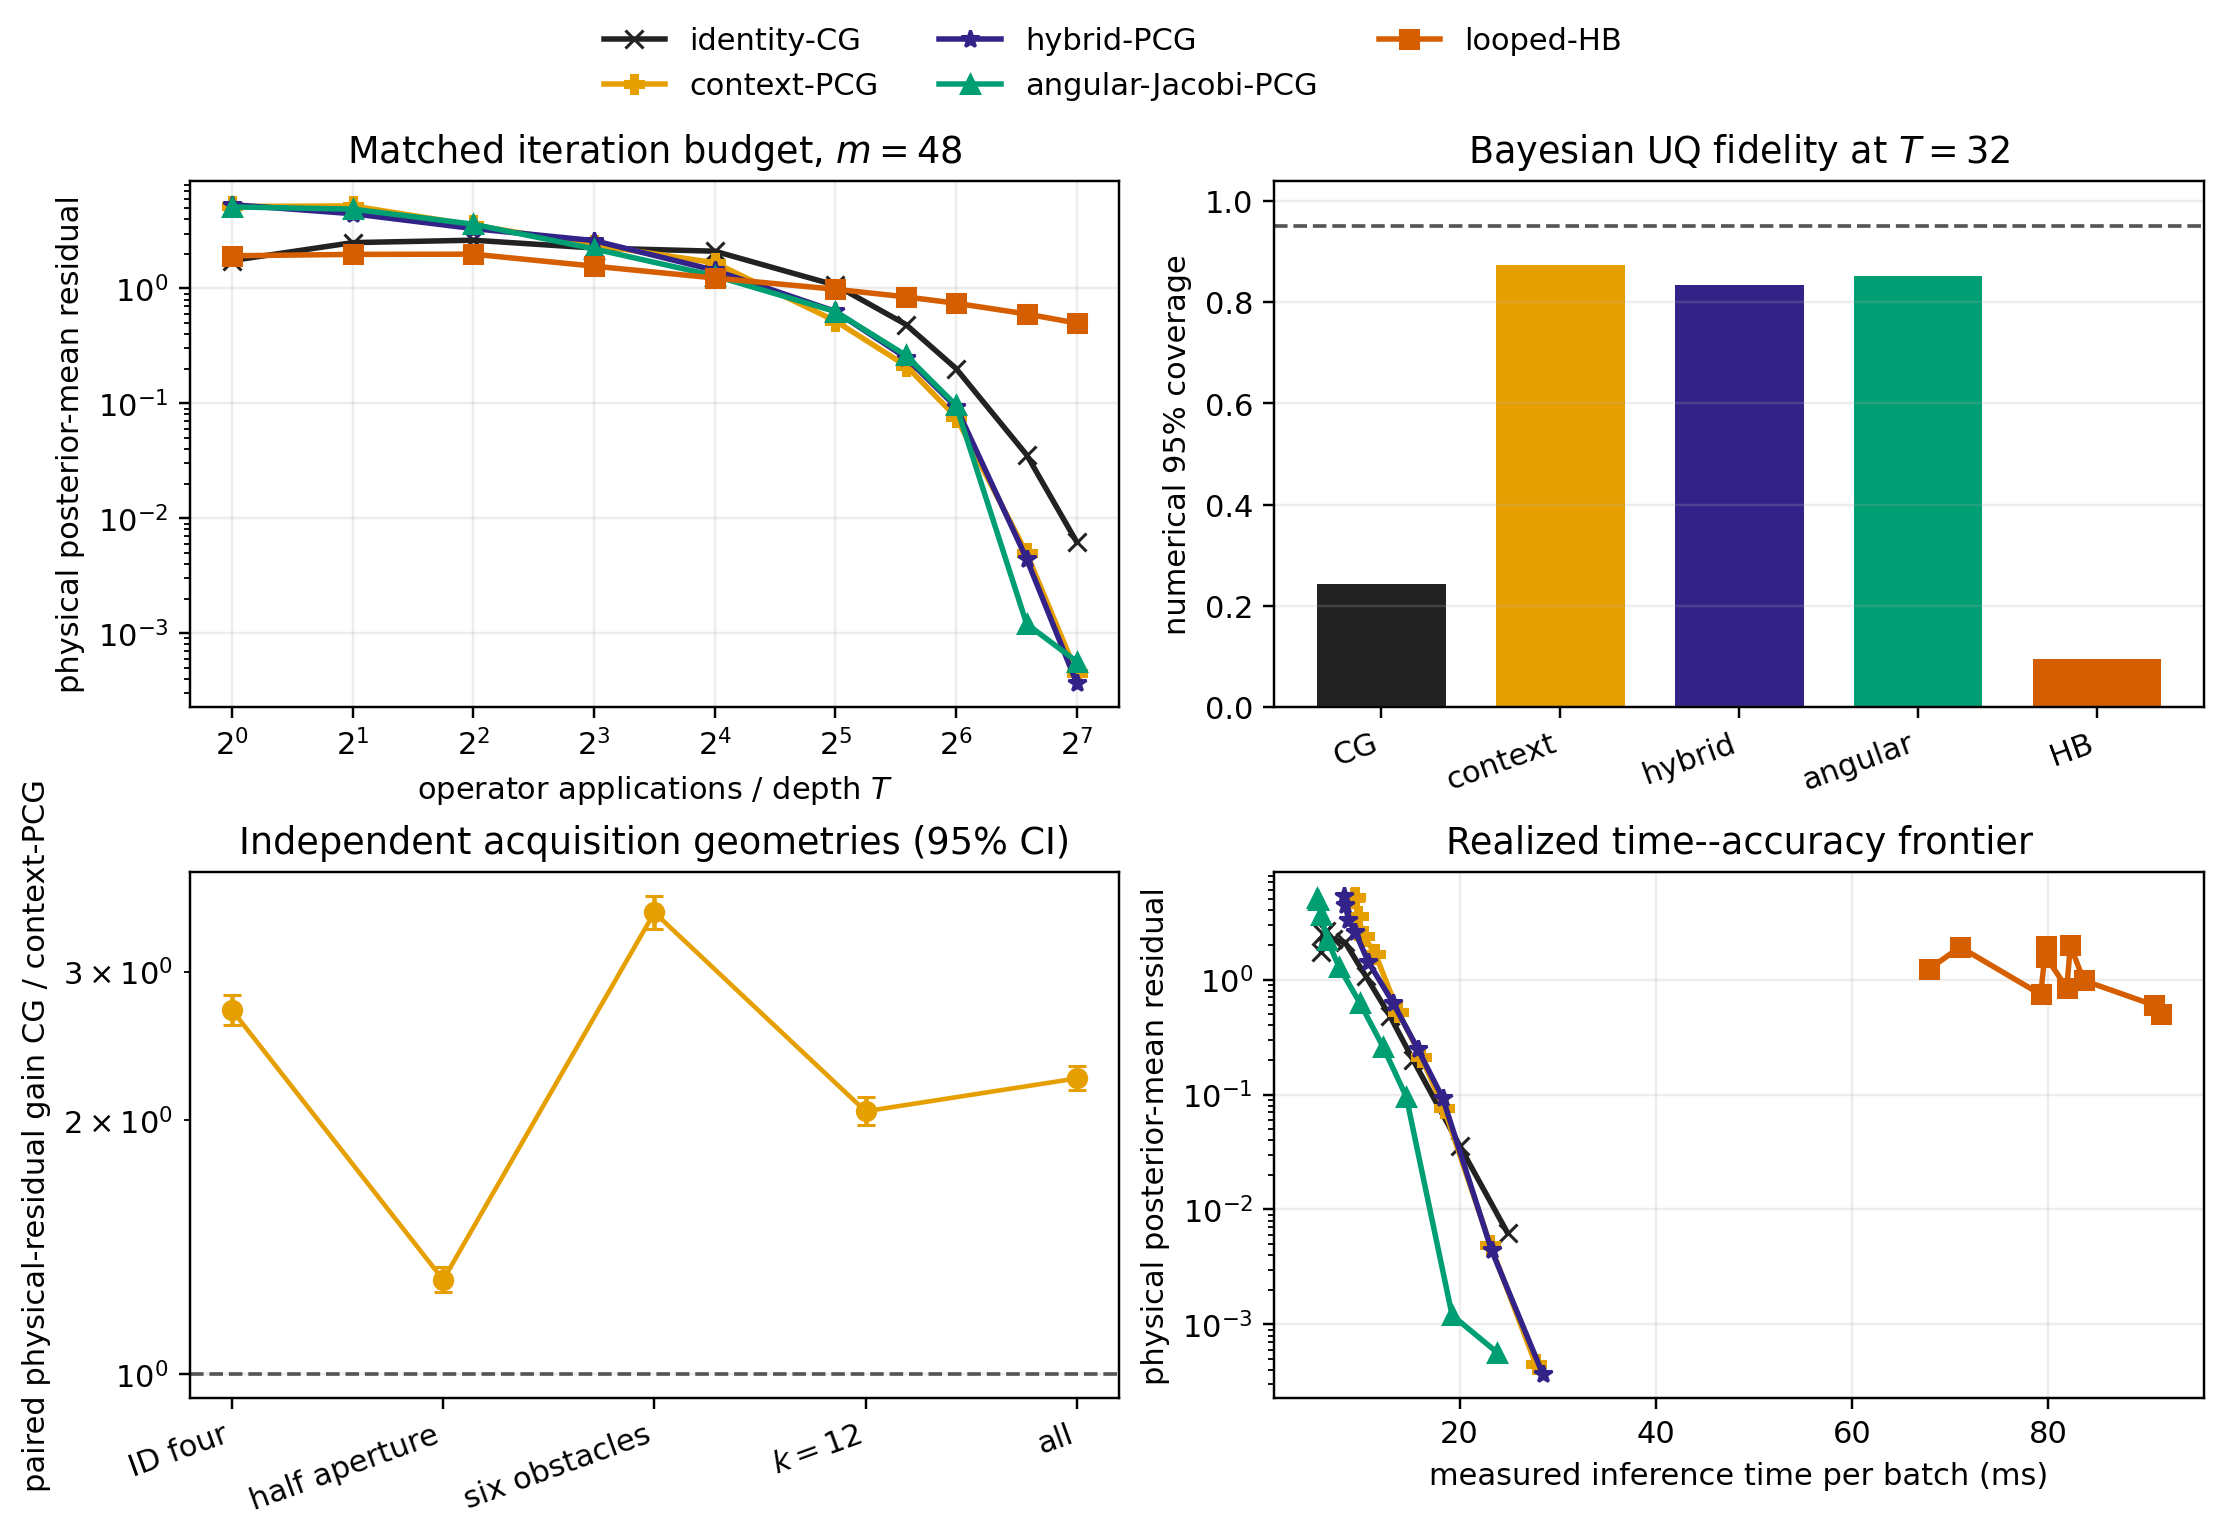
\includegraphics[width=0.70\linewidth]{scaling_cg_comparison.png}

\medskip
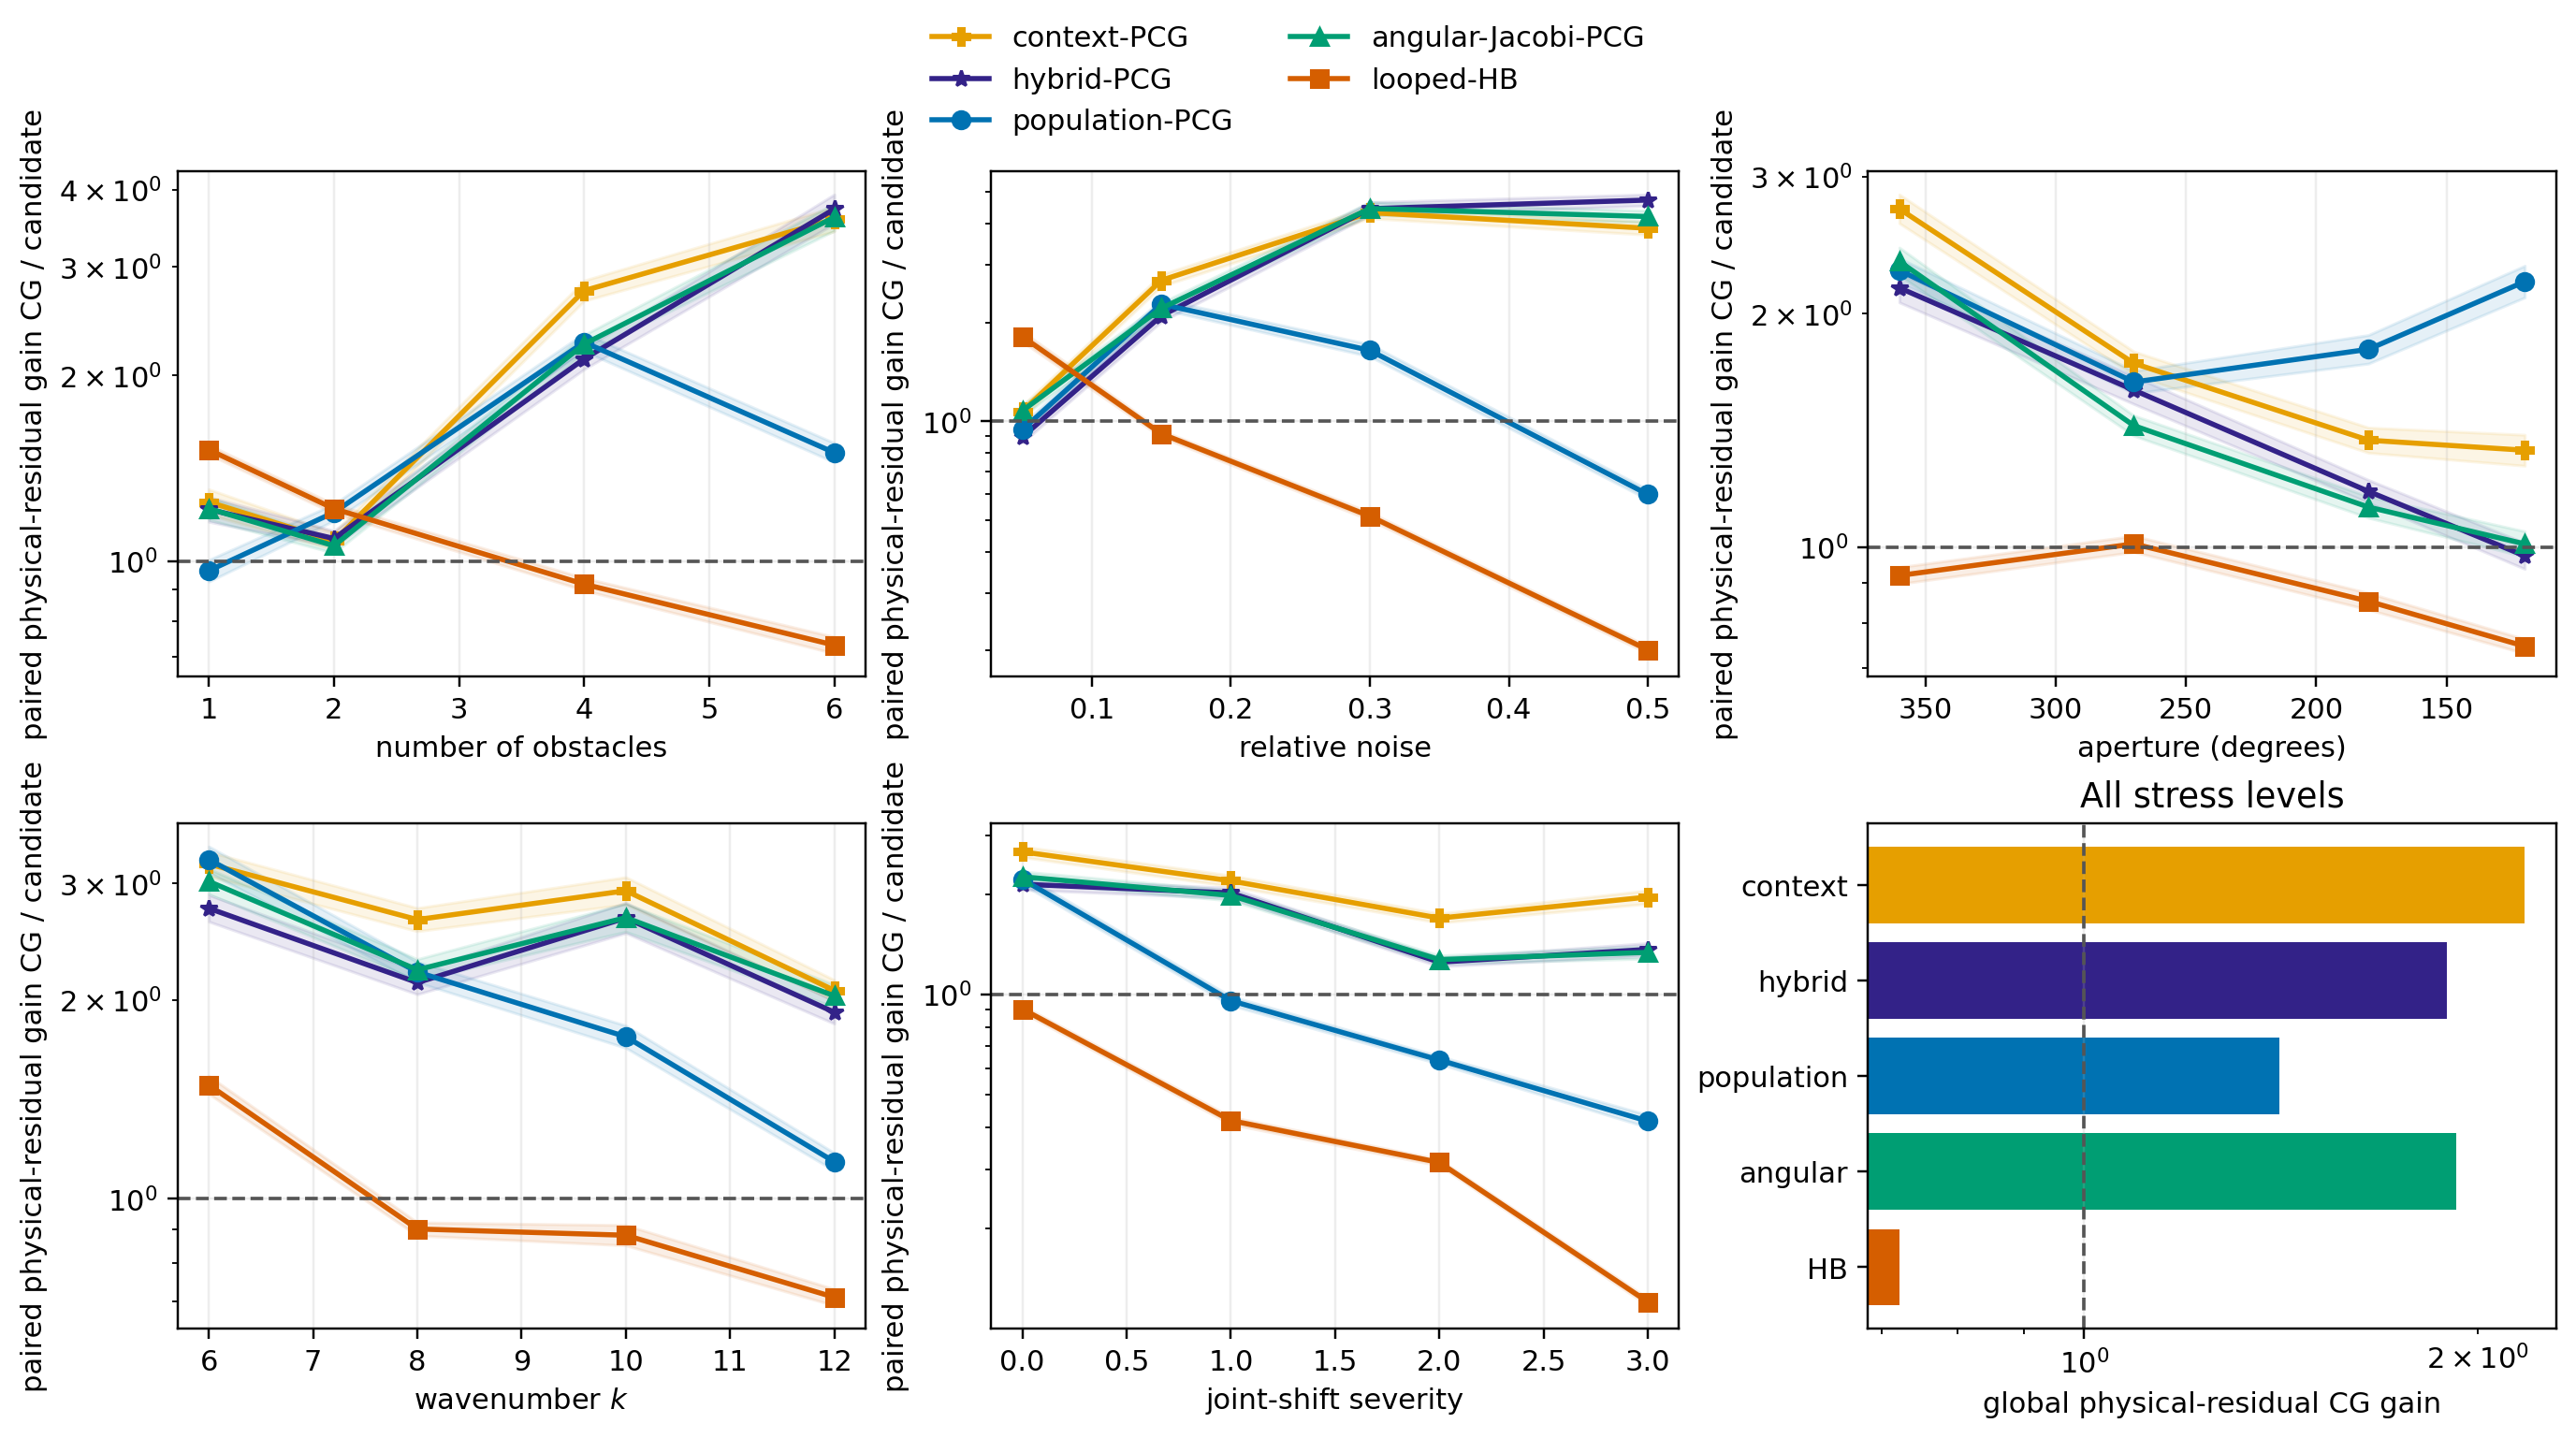
\includegraphics[width=0.70\linewidth]{scaling_cg_stress_test.png}
\caption{Top: direct physical-residual CG comparison at extrapolative context
$m=48$; the paired-geometry panel uses 768 batches.  Bottom: paired
physical-residual gains over
continuous physical stress axes, with 95\% mean-log-gain intervals.  Values
above one favor the preconditioned method over CG.}
\end{figure}

\end{document}
